% Provenance (never printed): see sources/outline_sources.md (Year 2: anatexis, migmatites,
% granite types and their sources). Wet granite solidus from Stern and Wyllie (1981) and
% Boettcher and Wyllie (1968); dehydration-melting brackets from Patino Douce and Harris
% (1998), Berger and Kalt (1999), Skjerlie and Johnston (1996); water solubility from Holtz
% et al. (1995); migmatite terms from the IUGS-SCMR proposal and BGS RR 99-02; aluminosity
% after Shand (as given by Moyen et al. 2017); figure data in figdata/bachelor-2/anatexis.py
% (paths from ptpaths.py); exercise and problem values in the Book 4 scratch calculator
% calc/ch12.py.
\chapter{Fusion de la croûte~: migmatites et granites}\label{ch:b2:crustal-melting}

Le granite est ce qui rend les continents légers, et le manteau ne peut pas le
produire directement~: les liquides de la \omterm{def:b2:mantle-melting:peridotites}{péridotite} sont des basaltes. Presque tout
le granite est la croûte continentale qui fond elle-même. Lorsqu'une racine de montagne
épaissie chauffe, lorsque du basalte s'accumule sous la croûte, ou lorsqu'une roche chaude
remonte et que sa pression baisse, les micas et les amphiboles de la croûte profonde
abandonnent leur eau, un liquide granitique apparaît entre les grains, et la roche devient
une \omterm{def:b2:crustal-melting:migmatite}{migmatite}, moitié métamorphique, moitié magmatique. Ce chapitre suit ce liquide depuis
ses premiers films jusqu'au \omterm{def:b2:magma-emplacement:bodies}{pluton} qu'il peut bâtir, et lit dans la chimie d'un granite la roche d'où il vient.

\begin{recall}
\textbf{Du volume lycée}~: granite, granitoïde et granodiorite~; roches felsiques et mafiques~;
les racines des chaînes de montagnes. \textbf{Du volume de première année}~: production de chaleur radiogénique dans la croûte~;
l'hydrolyse des silicates et des minéraux argileux. \textbf{Des volumes de chimie}~: le solidus et le liquidus d'un système binaire,
masse molaire et quantité de matière. \textbf{Du
\cref{ch:b2:magma-emplacement}}~: \omterm{def:b2:magma-emplacement:bodies}{dykes}, \omterm{def:b2:magma-emplacement:bodies}{plutons} et \omterm{def:b2:magma-emplacement:ascent}{diapirs}. \textbf{Du
\cref{ch:b2:mantle-melting}}~: \omterm{def:b2:mantle-melting:melting}{fusion partielle}, \omterm{def:b2:mantle-melting:peritectic}{fusion incongruente} et \omterm{def:b2:mantle-melting:melting}{fusion
par décompression}. \textbf{Du \cref{ch:b2:metamorphic-facies}}~: \omterm{def:b2:metamorphic-facies:protoliths}{métapélites}, \omterm{def:b2:metamorphic-facies:clapeyron}{pente de Clapeyron} d'une
réaction et les faciès. \textbf{Du \cref{ch:b2:pt-paths}}~: \omterm{def:b2:pt-paths:ptt}{chemins P--T--t} et le
modèle d'épaississement de la croûte.
\end{recall}

\section{Pourquoi la croûte fond}\label{sec:b2:crustal-melting:why}

Le mot est ancien et simple.

\begin{definition}[Anatexie]\label{def:b2:crustal-melting:anatexis}
\emph{Anatexie}\index{anatexie} est la fusion d'une roche, quel que soit son degré de fusion~;
en pratique le mot désigne la \omterm{def:b2:mantle-melting:melting}{fusion partielle} de la croûte continentale.
\end{definition}
% ledger: scmr:migmatite

\subsection*{Le solidus humide}

Le granite ne fond à basse température que lorsqu'il est humide. Stern et Wyllie ont fondu un
granite à biotite du \omterm{def:b2:magma-emplacement:bodies}{batholite} de la Sierra Nevada en présence d'eau en excès~: le premier liquide apparaît
à \qty{680}{\celsius} sous \qty{2}{kbar} et à \qty{620}{\celsius} sous \qty{10}{kbar}, et la
roche entière n'est fondue qu'à \qty{35}{\celsius} au-dessus du solidus sous \qty{2}{kbar}, mais
à \qty{105}{\celsius} au-dessus sous \qty{10}{kbar}. Le même granite, étudié plus tôt par
Boettcher et Wyllie, commence à fondre à \qty{605}{\celsius} sous \qty{15.3}{kbar}~; vers
\qty{17}{kbar} son plagioclase se décompose en jadéite et quartz, et à partir de là le solidus
remonte, pour atteindre \qty{670}{\celsius} sous \qty{27}{kbar}.
% ledger: sw81:wet-solidus, bw68:wet-solidus

Le solidus humide descend lorsque la pression monte, à l'inverse d'un solidus sec. La raison tient à
l'endroit où va l'eau. L'eau libre est un fluide de faible densité~; dissoute dans le liquide, elle prend très
peu de place~: Holtz et ses collaborateurs ont trouvé que son volume molaire partiel dans un liquide
granitique est voisin de \qtyrange{10}{12}{\cubic\centi\metre\per\mole}, contre \qty{18}{\cubic\centi\metre\per\mole}
pour l'eau liquide dans les conditions ambiantes, et davantage pour un fluide chaud. La réaction de fusion
\[\text{quartz} + \text{feldspaths} + \ce{H2O}\ (\text{fluide}) \longrightarrow
\text{liquide hydraté}\]
présente donc une variation de volume négative, alors que sa variation d'entropie, comme pour toute fusion,
est positive~: par la relation de Clapeyron du \cref{ch:b2:metamorphic-facies}, sa pente
$\mathrm{d}P/\mathrm{d}T = \Delta S/\Delta V$ est négative. La pression fait aussi entrer davantage d'eau
dans le liquide~: pour un liquide haplogranitique à \qty{800}{\celsius}, la teneur de saturation passe
de \qty{2.80}{\percent} en masse à \qty{0.5}{kbar} jusqu'à \qty{9.97}{\percent} à \qty{5}{kbar} et
\qty{13.82}{\percent} à \qty{8}{kbar}, soit environ \qty{1.27}{\percent} de plus par kilobar entre 3 et
\qty{8}{kbar}.
% ledger: holtz95:solubility

\begin{omfigure}
\centering
\begin{tikzpicture}
\begin{axis}[omrecord, width=0.5\linewidth, height=4.8cm,
  xmin=0, xmax=9, ymin=0, ymax=15, xlabel={$P$ (\unit{kbar})},
  ylabel={\ce{H2O} dans le liquide (\unit{\percent})},
  tick label style={font=\scriptsize}, label style={font=\small}]
\addplot[only marks, mark=*, mark size=1.6pt, blue!70!black]
  table[x=P_kbar, y=H2O_wt] {figdata/out/bachelor-2-anatexis-water.dat};
\addplot[thick, red!75!black] table[x=P_kbar, y=H2O_wt] {figdata/out/bachelor-2-anatexis-waterfit.dat};
\end{axis}
\end{tikzpicture}
\par\smallskip{\small Eau qu'un liquide haplogranitique peut dissoudre à \qty{800}{\celsius}
(points mesurés)~; rouge~: la droite des moindres carrés passant par les points de 3 à
\qty{8}{kbar}, de pente \qty{1.26}{\percent} par kilobar.}
\end{omfigure}
% ledger: holtz95:solubility

Mais la croûte profonde contient peu d'eau libre~: une roche métamorphique chauffée a
déjà expulsé l'essentiel de son eau interstitielle par les réactions de déshydratation du
\cref{ch:b2:metamorphic-facies}. Son eau est désormais enfermée dans les micas et les amphiboles. La
fusion doit alors attendre que ces minéraux eux-mêmes se décomposent.

\begin{definition}[Fusion en présence de fluide et fusion par déshydratation]\label{def:b2:crustal-melting:reactions}
\emph{Fusion en présence de fluide}\index{fusion en présence de fluide} (ou \omterm{def:b2:mantle-melting:melting}{fusion hydratée}) est
la fusion en présence d'un fluide aqueux libre, au voisinage du solidus humide~; le liquide
produit est limité par l'apport de fluide. \emph{Fusion par déshydratation}\index{fusion par déshydratation}
(fusion en l'absence de fluide) est la \omterm{def:b2:mantle-melting:peritectic}{fusion incongruente} d'un minéral hydraté, mica ou
amphibole, avec du quartz et du feldspath, sans fluide libre~: l'eau du minéral
passe dans le liquide, et de nouveaux minéraux anhydres (feldspath potassique péritectique, alumino-silicate,
grenat, cordiérite, orthopyroxène) croissent à côté.
\end{definition}
% ledger: pj98:productivity, koester02:melting, pdh98:himalaya

Les expériences fixent l'endroit où chaque minéral hydraté cède. Dans les schistes à muscovite de l'Himalaya,
Patiño Douce et Harris observent une \omterm{def:b2:crustal-melting:reactions}{fusion par déshydratation} qui commence entre 750 et \qty{800}{\celsius}
pour 6 à \qty{10}{kbar}~; de l'eau ajoutée aux mêmes roches abaisse le solidus, mais donne des liquides
trondhjémitiques, différents des \omterm{def:b2:crustal-melting:leucogranite}{leucogranites}. Un gneiss semi-pélitique commence à fondre vers
\qty{700}{\celsius} grâce à sa muscovite phengitique, mais ne produit pas plus de \qty{9}{\percent} de liquide~; au-dessus de
\qty{800}{\celsius}, la décomposition de la biotite et de la cordiérite donne de 10 à
\qty{63}{\percent} de liquide en volume.
La \omterm{def:b2:crustal-melting:reactions}{fusion par déshydratation} de la biotite a lieu de 800 à \qty{850}{\celsius} et de
\qty{0.5}{GPa} à \qty{0.7}{GPa} dans les \omterm{def:b2:crustal-melting:migmatite}{migmatites} de la Bayerische Wald, et l'amphibole
ajoute environ \qty{25}{\percent} de liquide en volume entre 875 et \qty{925}{\celsius}, sous 10 à
\qty{12.5}{kbar}. L'ordre est celui de la tenue de l'eau~: la muscovite d'abord, la biotite ensuite, l'amphibole en dernier.
% ledger: pdh98:himalaya, koester02:melting, bk99:migmatites, sj96:amphibole, moyen17:aluminosity

\begin{proposition}[Un taux de fusion limité par l'eau]\label{prop:b2:crustal-melting:water}
Dans une \omterm{def:b2:crustal-melting:reactions}{fusion par déshydratation} sans fluide libre, si une roche contient une fraction massique $X$
d'un minéral hydraté qui contient une fraction massique $w$ d'eau, et si toute cette eau passe dans un liquide
qui contient une fraction massique $c$ d'eau, la fraction massique de liquide vaut
\[F = \frac{X\,w}{c}.\]
Comme $c$ ne peut dépasser la teneur de saturation $c_{\mathrm{sat}}$
à la pression et à la température de fusion, $F \ge X\,w/c_{\mathrm{sat}}$~:
moins le liquide contient d'eau, plus le même mica produit de liquide.
\end{proposition}

\begin{proof}
Par kilogramme de roche, le minéral libère $X\,w$ kilogrammes d'eau. Sans phase fluide ni eau restant dans les solides,
toute cette eau se retrouve dans le liquide, dont la masse $F$ contient $c\,F$
kilogrammes d'eau~: $c\,F = X\,w$. Comme $c \le c_{\mathrm{sat}}$, $F = Xw/c \ge
Xw/c_{\mathrm{sat}}$.
\end{proof}

Une muscovite, \ce{KAl3Si3O10(OH)2} de masse molaire \qty{398.3}{\gram\per\mole}, porte deux groupes
hydroxyle, soit l'équivalent d'une molécule d'eau, soit \qty{4.52}{\percent} de sa masse. Un schiste à
\qty{20}{\percent} de muscovite contient donc \qty{9.0}{\gram} d'eau par kilogramme à céder~; dissoute
à \qty{6}{\percent}, cette eau forme \qty{150}{\gram} de liquide. Les micas fixent le budget, et c'est
pourquoi la croûte fertile, celle qui fond facilement, est riche en mica~:
les \omterm{def:b2:metamorphic-facies:protoliths}{métapélites} en premier.

\begin{omfigure}
\centering
\begin{tikzpicture}
\begin{axis}[omrecord, width=0.8\linewidth, height=7cm,
  xmin=500, xmax=1000, ymin=0, ymax=20, xlabel={$T$ (\unit{\celsius})}, ylabel={$P$ (\unit{kbar})},
  tick label style={font=\scriptsize}, label style={font=\small}, clip=false]
\addplot[fill=orange!35, draw=orange!70!black] coordinates {(750,6) (800,6) (800,10) (750,10) (750,6)};
\addplot[fill=red!25, draw=red!70!black] coordinates {(800,5) (850,5) (850,7) (800,7) (800,5)};
\addplot[fill=green!25, draw=green!50!black] coordinates {(875,10) (925,10) (925,12.5) (875,12.5) (875,10)};
\node[font=\scriptsize, orange!50!black, align=center] at (axis cs:775,8) {mus-\\covite};
\node[font=\scriptsize, red!60!black] at (axis cs:825,4.4) {biotite};
\node[font=\scriptsize, green!35!black, anchor=west] at (axis cs:927,11.25) {amphibole};
\addplot[very thick, blue!70!black, mark=*, mark size=1.5pt]
  table[x=T_C, y=P_kbar] {figdata/out/bachelor-2-anatexis-solidi.dat};
\node[font=\scriptsize, blue!70!black, anchor=west] at (axis cs:612,15.6) {solidus humide du granite};
\addplot[thick, black, postaction={decorate}, decoration={markings,
  mark=at position 0.3 with {\arrow{>}}, mark=at position 0.75 with {\arrow{>}}}]
  table[x=T_C, y=P_kbar, restrict x to domain=500:1000,
  restrict expr to domain={\thisrow{t_Myr}}{0:100}] {figdata/out/bachelor-2-anatexis-path35.dat};
\node[font=\scriptsize, anchor=north] at (axis cs:560,4.2) {roche issue de \qty{35}{km}};
\addplot[thick, dashed, black, postaction={decorate}, decoration={markings,
  mark=at position 0.3 with {\arrow{>}}, mark=at position 0.7 with {\arrow{>}}}]
  table[x=T_C, y=P_kbar, restrict x to domain=500:1000,
  restrict expr to domain={\thisrow{t_Myr}}{0:100}] {figdata/out/bachelor-2-anatexis-path70.dat};
\node[font=\scriptsize, anchor=south] at (axis cs:760,19.4) {base de la croûte épaissie};
\end{axis}
\end{tikzpicture}
\par\smallskip{\small Où la croûte fond. Bleu~: le solidus d'un granite à biotite en présence d'eau en excès
(points mesurés, reliés par des segments droits). Encadrés~: les conditions auxquelles la \omterm{def:b2:crustal-melting:reactions}{fusion par
déshydratation} de la muscovite, de la biotite et de l'amphibole a été observée dans des expériences et dans
des \omterm{def:b2:crustal-melting:migmatite}{migmatites}. Noir~: trajets calculés avec le modèle d'épaississement du
\cref{ch:b2:pt-paths}~; la roche qui se retrouve à \qty{35}{km} après l'empilement (trait plein) n'atteint jamais
le solidus humide, tandis que la base de la croûte épaissie (tirets) dépasse
\qty{900}{\celsius}. Les deux trajets sont tracés pour les 100 premiers Ma, jusqu'à l'arrêt de
l'érosion.}
\end{omfigure}
% ledger: sw81:wet-solidus, bw68:wet-solidus, pdh98:himalaya, bk99:migmatites, sj96:amphibole, et84:ptt

\subsection*{D'où vient la chaleur}

La figure ci-dessus pose le problème~: la croûte ne fond que là où elle dépasse environ
\qty{700}{\celsius}, alors que le géotherme stationnaire du modèle du \cref{ch:b2:pt-paths}
n'atteint que \qty{595}{\celsius} à la base d'une croûte de \qty{35}{km}. Trois voies mènent
au-delà des réactions de \omterm{def:b2:crustal-melting:reactions}{fusion par déshydratation}.

\emph{Épaississement et chaleur radiogénique.} Dans le modèle du \cref{ch:b2:pt-paths}, une croûte
doublée par empilement s'échauffe de l'intérieur~; la roche qui se retrouve à mi-profondeur de la croûte culmine à
\qty{593}{\celsius} et ne fond jamais, mais la base de la croûte épaissie dépasse
\qty{800}{\celsius} au bout d'environ 31 Ma et \qty{900}{\celsius} au bout d'environ 56, au-delà de la réaction de la
biotite. La fusion de la croûte inférieure est une conséquence lente de l'épaississement.
% ledger: et84:ptt

\emph{Décompression.} Une roche chaude remontée plus vite qu'elle ne se refroidit traverse les
courbes de \omterm{def:b2:crustal-melting:reactions}{fusion par déshydratation} par le côté des hautes pressions. Patiño Douce et Harris ont
trouvé que le solidus du schiste à muscovite a une pente $\mathrm{d}P/\mathrm{d}T$ plus petite que celui du schiste à biotite, si bien que le schiste à muscovite fond plus facilement par décompression, et ils
ont conclu que les \omterm{def:b2:crustal-melting:leucogranite}{leucogranites} himalayens se sont formés par \omterm{def:b2:crustal-melting:reactions}{fusion par déshydratation} de \omterm{def:b2:metamorphic-facies:protoliths}{métapélites}
pendant une décompression adiabatique de 6 à \qty{8}{kbar} et de 750 à
\qty{770}{\celsius}.
% ledger: pdh98:himalaya

\emph{Chaleur venue du dessous.} Du basalte issu du manteau, arrêté à la base de la croûte, apporte
avec lui sa chaleur et sa chaleur latente de cristallisation.

\begin{definition}[Sous-placage basique]\label{def:b2:crustal-melting:underplating}
\emph{Sous-placage basique}\index{sous-placage basique} est l'accumulation d'un \omterm{def:b2:magma-emplacement:magma}{magma} basaltique issu du manteau
à la base, ou près de la base, de la croûte continentale, où il cristallise et
libère sa chaleur dans la croûte qui le surmonte.
\end{definition}

Le sous-placage a été invoqué, par exemple, pour les rhyolites de la péninsule Antarctique,
où un \omterm{def:b2:magma-emplacement:magma}{magma} andésitique à dacitique est issu de la fusion de la croûte inférieure basique hydratée en réponse au
sous-placage~; des liquides mantelliques peuvent aussi former eux-mêmes des granitoïdes, en cristallisant
ou en refondant des corps récemment sous-plaqués.
% ledger: riley01:underplating, moyen17:settings, johansson23:a-type

\begin{proposition}[Bilan thermique du sous-placage]\label{prop:b2:crustal-melting:heat}
Un volume $V_b$ de basalte intrudé à $T_b$, qui cristallise complètement en libérant une chaleur latente $L_b$
par unité de volume, et refroidit jusqu'à $T_f$, peut porter un volume $V_c$ de croûte de $T_c$ à $T_f$
et y faire fondre une fraction $F$, avec
\[\frac{V_c}{V_b} = \frac{L_b + C\,(T_b - T_f)}{C\,(T_f - T_c) + F\,L_c},\]
où $C$ est la capacité calorifique par unité de volume (supposée égale pour les deux roches) et $L_c$ la
chaleur latente du liquide crustal par unité de volume, en l'absence de perte de chaleur.
\end{proposition}

\begin{proof}
La chaleur dégagée par le basalte, $V_b[L_b + C(T_b - T_f)]$, égale la chaleur absorbée par la
croûte, $V_c[C(T_f - T_c) + F L_c]$~; on divise par $V_b$ puis par le crochet de la croûte.
\end{proof}

Avec $C = \qty{2.5}{\mega\joule\per\cubic\metre\per\kelvin}$ et des chaleurs latentes de
\qty{900}{\mega\joule\per\cubic\metre}, valeurs typiques des \omterm{def:b2:magma-emplacement:magma}{magmas}, un basalte qui refroidit de
\qty{1200}{\celsius} à \qty{850}{\celsius} peut chauffer environ deux fois et demie son volume de
croûte à partir de \qty{650}{\celsius} et en faire fondre un cinquième (voir l'\cref{exo:b2:crustal-melting:7}).
Le sous-placage est efficace, mais local~: la chaleur va là où se trouve le basalte.
% ledger: delaney86b4:properties

\section{Anatexie et migmatites}\label{sec:b2:crustal-melting:migmatites}

Une roche partiellement fondue qui se fige avant que son liquide ne s'en aille garde ses deux parties côte à côte.

\begin{definition}[Migmatite et ses parties]\label{def:b2:crustal-melting:migmatite}
Une \emph{migmatite}\index{migmatite} est une roche silicatée composite,
hétérogène à l'échelle de l'affleurement, faite de parties sombres d'aspect métamorphique
et de parties claires d'aspect plutonique. Son \emph{leucosome}\index{leucosome} est sa partie claire,
riche en quartz et en feldspath~; son \emph{mélanosome}\index{mélanosome} sa partie sombre, riche en
minéraux sombres, complémentaire du leucosome~; son \emph{mésosome}, la partie de couleur intermédiaire,
relique plus ou moins modifiée de la roche mère (le \emph{paléosome}). Le leucosome et le mélanosome
forment ensemble le \emph{néosome}, la partie nouvellement formée. Une \emph{métatexite}\index{métatexite}
est une migmatite aux leucosomes, mésosomes et mélanosomes discrets et bien délimités~; une
\emph{diatexite}\index{diatexite} est une migmatite dont les parties claires et sombres se fondent en
stries (schlieren) et en structures fantomatiques (nébulitiques).
\end{definition}
% ledger: scmr:migmatite, bgs99:migmatite

La définition est volontairement descriptive~: qu'un \omterm{def:b2:crustal-melting:migmatite}{leucosome} soit un liquide figé, un liquide venu
d'ailleurs ou une ségrégation métamorphique est une interprétation. Lorsqu'il s'agit d'un liquide,
le \omterm{def:b2:crustal-melting:migmatite}{leucosome} est ce liquide et le \omterm{def:b2:crustal-melting:migmatite}{mélanosome} le résidu solide qu'il a laissé, enrichi en biotite,
grenat ou cordiérite~: une \omterm{def:b2:crustal-melting:migmatite}{métatexite} témoigne du premier stade de l'\omterm{def:b2:crustal-melting:anatexis}{anatexie}, où seule une partie
de la roche a fondu, et une \omterm{def:b2:crustal-melting:migmatite}{diatexite} d'un stade avancé, où les minéraux sombres ont fondu eux aussi
et où le liquide est resté en place.
% ledger: scmr:migmatite

Quelle quantité de liquide contient une \omterm{def:b2:crustal-melting:migmatite}{migmatite}~? Dans les \omterm{def:b2:crustal-melting:migmatite}{migmatites} à cordiérite du Bayerische Wald,
formées par \omterm{def:b2:crustal-melting:reactions}{fusion par déshydratation} de la biotite, les \omterm{def:b2:crustal-melting:migmatite}{leucosomes} qui sont du liquide ancien pur représentent 20 à
\qty{40}{\percent} de la roche en volume, proche des 20 à \qty{30}{\percent} produits dans les expériences de
\omterm{def:b2:crustal-melting:reactions}{fusion par déshydratation} sur des roches voisines dans les mêmes conditions~; là où le liquide a été extrait, comme dans
les types les plus déformés, le résidu reste sur place.
% ledger: bk99:migmatites

\begin{inthefield}[Lire un affleurement de migmatite]
Sur un affleurement de \omterm{def:b2:crustal-melting:migmatite}{migmatite}, un géologue commence par cartographier les parties et leur géométrie~: si les
\omterm{def:b2:crustal-melting:migmatite}{leucosomes} sont parallèles à la foliation ou la recoupent, s'ils portent une bordure mélanocrate sombre,
et quelle quantité de \omterm{def:b2:crustal-melting:migmatite}{mélanosome} accompagne chaque \omterm{def:b2:crustal-melting:migmatite}{leucosome}. Chaque trait a une signification. Une roche
résiduelle, mélanocrate, marque l'endroit d'où vient le liquide~; des \omterm{def:b2:crustal-melting:migmatite}{leucosomes} minces, courts et ramifiés,
avec peu de \omterm{def:b2:crustal-melting:migmatite}{mélanosome}, marquent une fusion qui vient de commencer~; des \omterm{def:b2:crustal-melting:migmatite}{leucosomes} parallèles à la foliation
marquent l'endroit où le liquide s'est écoulé de la matrice et s'est rassemblé~; des \omterm{def:b2:crustal-melting:migmatite}{leucosomes} à grand angle
avec la stratification, sans bordure sombre en général, se sont formés en dernier et marquent les canaux par lesquels
le liquide est sorti. Un fort rapport \omterm{def:b2:crustal-melting:migmatite}{mélanosome} sur \omterm{def:b2:crustal-melting:migmatite}{leucosome} signifie que l'essentiel du liquide est parti.
Des échantillons de \omterm{def:b2:crustal-melting:migmatite}{leucosome}, de \omterm{def:b2:crustal-melting:migmatite}{mélanosome} et de mésosome sont ensuite prélevés pour analyse, afin de tester par bilan
de masse si l'affleurement a perdu du liquide (voir l'\cref{exo:b2:crustal-melting:12}).
\end{inthefield}
% ledger: sawyer01:segregation, bgs99:migmatite, scmr:migmatite

\begin{omfigure}
\centering
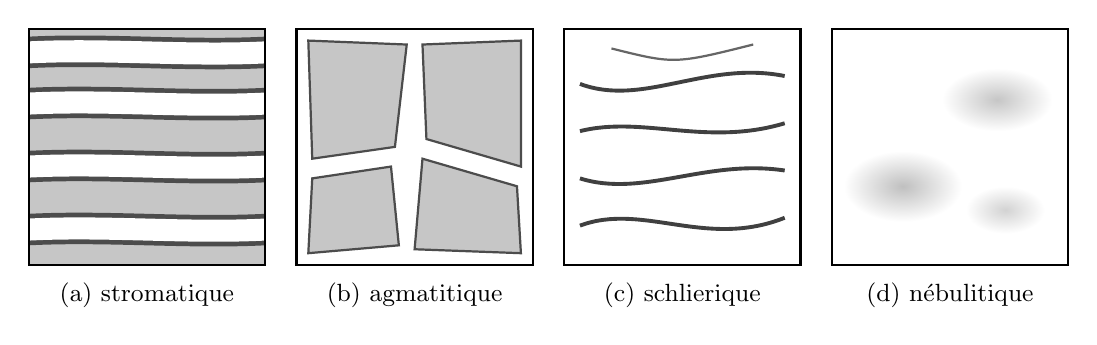
\begin{tikzpicture}[x=1cm, y=1cm]
% (a) stromatic
\begin{scope}
\fill[gray!45] (0,0) rectangle (3,3);
\foreach \y in {0.45, 1.25, 2.05, 2.7} {
  \fill[black!70] (0,\y-0.2) .. controls (1,\y-0.15) and (2,\y-0.25) .. (3,\y-0.2)
    -- (3,\y+0.2) .. controls (2,\y+0.15) and (1,\y+0.25) .. (0,\y+0.2) -- cycle;
  \fill[white] (0,\y-0.14) .. controls (1,\y-0.09) and (2,\y-0.19) .. (3,\y-0.14)
    -- (3,\y+0.14) .. controls (2,\y+0.09) and (1,\y+0.19) .. (0,\y+0.14) -- cycle;
}
\draw[thick] (0,0) rectangle (3,3);
\node[font=\small, anchor=north] at (1.5,-0.1) {(a) stromatique};
\end{scope}
% (b) agmatitic
\begin{scope}[xshift=3.4cm]
\fill[white] (0,0) rectangle (3,3);
\fill[gray!45, draw=black!70, thick] (0.15,0.15) -- (1.3,0.25) -- (1.2,1.25) -- (0.2,1.1) -- cycle;
\fill[gray!45, draw=black!70, thick] (1.5,0.2) -- (2.85,0.15) -- (2.8,1.0) -- (1.6,1.35) -- cycle;
\fill[gray!45, draw=black!70, thick] (0.2,1.35) -- (1.25,1.5) -- (1.4,2.8) -- (0.15,2.85) -- cycle;
\fill[gray!45, draw=black!70, thick] (1.65,1.6) -- (2.85,1.25) -- (2.85,2.85) -- (1.6,2.8) -- cycle;
\draw[thick] (0,0) rectangle (3,3);
\node[font=\small, anchor=north] at (1.5,-0.1) {(b) agmatitique};
\end{scope}
% (c) schlieric
\begin{scope}[xshift=6.8cm]
\fill[white] (0,0) rectangle (3,3);
\foreach \y/\a in {0.5/0.3, 1.1/-0.25, 1.7/0.2, 2.3/-0.3} {
  \draw[black!75, line width=1.4pt] (0.2,\y) .. controls (1,\y+\a) and (1.8,\y-\a) .. (2.8,\y+0.1);
}
\draw[black!60, line width=0.8pt] (0.6,2.75) .. controls (1.4,2.55) .. (2.4,2.8);
\draw[thick] (0,0) rectangle (3,3);
\node[font=\small, anchor=north] at (1.5,-0.1) {(c) schlierique};
\end{scope}
% (d) nebulitic
\begin{scope}[xshift=10.2cm]
\fill[white] (0,0) rectangle (3,3);
\shade[inner color=gray!50, outer color=white] (0.9,1.0) ellipse (0.75 and 0.45);
\shade[inner color=gray!45, outer color=white] (2.1,2.1) ellipse (0.7 and 0.4);
\shade[inner color=gray!35, outer color=white] (2.2,0.7) ellipse (0.5 and 0.3);
\draw[thick] (0,0) rectangle (3,3);
\node[font=\small, anchor=north] at (1.5,-0.1) {(d) nébulitique};
\end{scope}
\end{tikzpicture}
\par\smallskip{\small Quatre structures de \omterm{def:b2:crustal-melting:migmatite}{migmatites}, schématiques (faces d'affleurement d'environ un mètre
de côté). Blanc~: \omterm{def:b2:crustal-melting:migmatite}{leucosome}~; noir~: \omterm{def:b2:crustal-melting:migmatite}{mélanosome}~; gris~: mésosome. (a) Stromatique~: couches de
\omterm{def:b2:crustal-melting:migmatite}{leucosome}, chacune avec une bordure sombre, parallèles à la foliation, typiques des \omterm{def:b2:crustal-melting:migmatite}{métatexites}.
(b) Agmatitique~: un réseau de veines de \omterm{def:b2:crustal-melting:migmatite}{leucosome} autour de blocs anguleux, d'aspect bréchique.
(c) Schlierique~: stries de minéraux sombres dans le \omterm{def:b2:crustal-melting:migmatite}{leucosome}. (d) Nébulitique~: fantômes diffus
de la roche antérieure dans un hôte d'aspect magmatique~; (c) et (d)
sont typiques des \omterm{def:b2:crustal-melting:migmatite}{diatexites}.}
\end{omfigure}
% ledger: bgs99:migmatite, scmr:migmatite

\begin{omfigure}
\centering
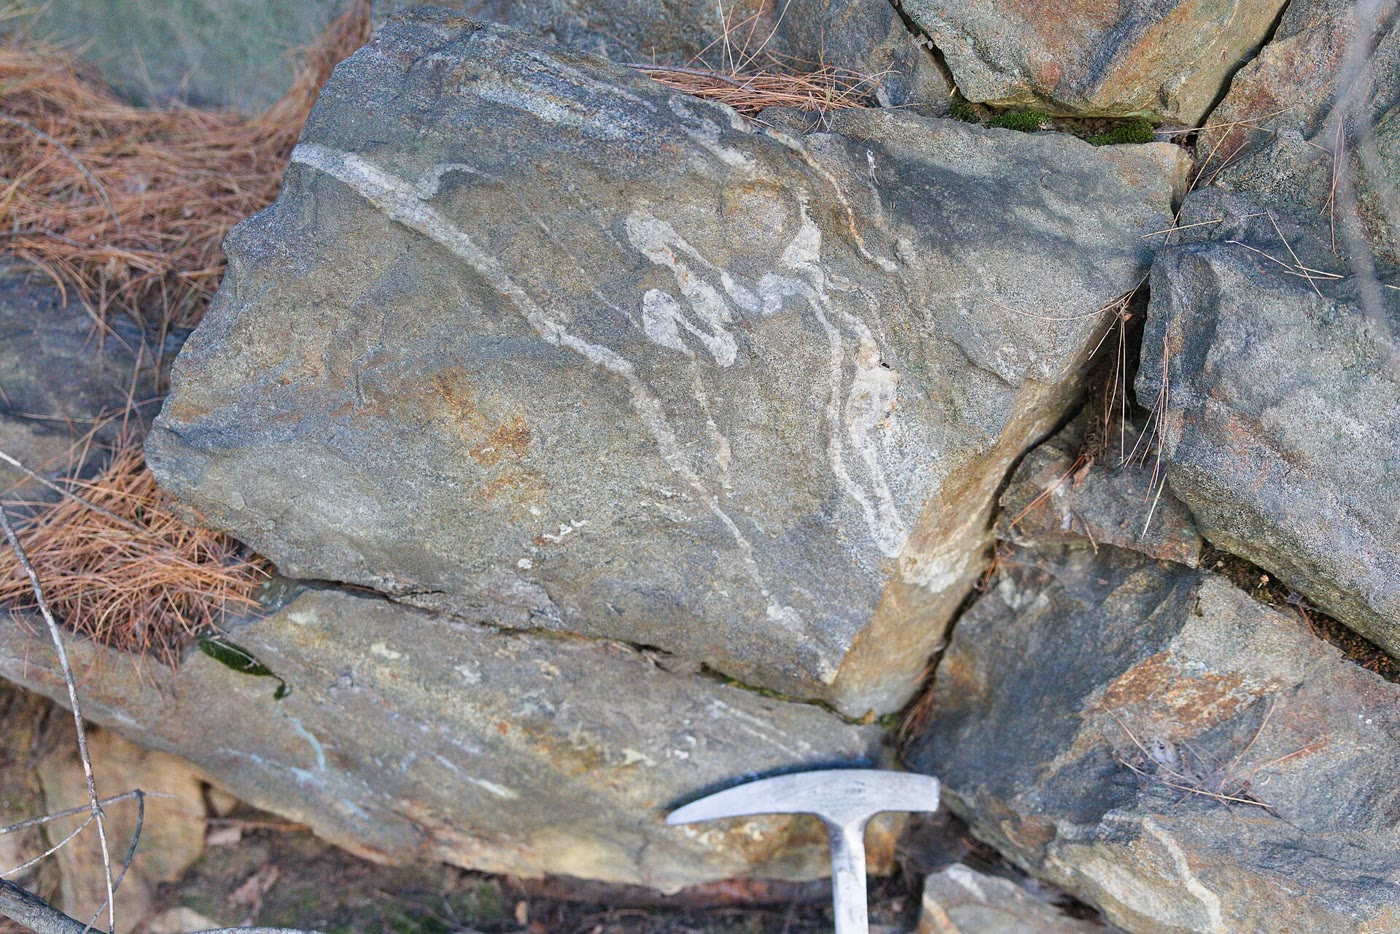
\includegraphics[width=0.62\linewidth]{images/book4/b2-12-migmatite.jpg}
\par\smallskip{\small Une \omterm{def:b2:crustal-melting:migmatite}{migmatite} à Nashua, New Hampshire~: veines claires de \omterm{def:b2:crustal-melting:migmatite}{leucosome}, plissées
avec le gneiss gris qui les porte. Le marteau du géologue donne l'échelle. Photographie Kevin M. Gill, CC BY 4.0.}
\end{omfigure}

\section{De la migmatite au pluton}\label{sec:b2:crustal-melting:segregation}

À l'échelle du grain, le premier liquide se loge le long des joints de grains et en petites poches,
surtout parallèlement à la foliation. Si petit soit-il, il modifie la roche~: dans des expériences sur un granite partiellement
fondu, la résistance de l'agrégat chute fortement entre le solidus et un \omterm{def:b2:mantle-melting:fraction}{taux de fusion} de \num{0.07},
au fur et à mesure que les joints de grains porteurs de liquide se connectent, puis chute encore,
d'environ quatre ordres de grandeur mais à partir d'une valeur déjà faible, quand l'ossature cristalline se rompt
aux \omterm{def:b2:mantle-melting:fraction}{taux de fusion} plus élevés. La croûte partiellement fondue est donc faible, et la déformation s'y concentre
dès que la fusion commence. La déformation à son tour entraîne le liquide~: il s'écoule de la matrice par des joints
de grains connectés vers des \omterm{def:b2:crustal-melting:migmatite}{leucosomes} parallèles à la foliation, puis hors de la couche en fusion par des \omterm{def:b2:crustal-melting:migmatite}{leucosomes}
qui la recoupent, et
ceux-ci se rejoignent en \omterm{def:b2:magma-emplacement:bodies}{dykes} du \cref{ch:b2:magma-emplacement}. La figure ci-dessous résume
le trajet de la source jusqu'au \omterm{def:b2:magma-emplacement:bodies}{pluton}.
% ledger: sawyer01:segregation, rh05:connectivity

\begin{omfigure}
\centering
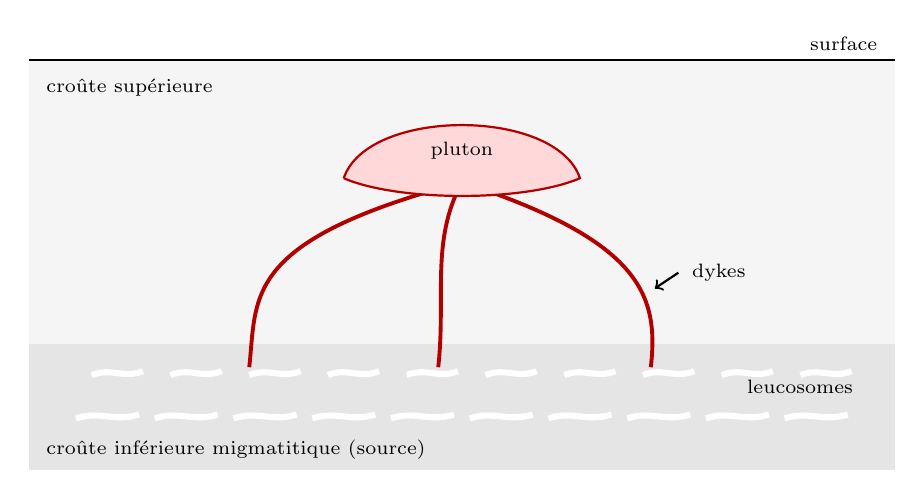
\begin{tikzpicture}[x=1cm, y=1cm]
\fill[gray!20] (0,0) rectangle (11,1.6);
\fill[gray!8] (0,1.6) rectangle (11,5.2);
\node[font=\scriptsize, anchor=west] at (0.1,0.25) {croûte inférieure migmatitique (source)};
\foreach \x in {0.6,1.6,2.6,3.6,4.6,5.6,6.6,7.6,8.6,9.6} {
  \draw[white, line width=2.2pt] (\x,0.65) .. controls (\x+0.3,0.75) and (\x+0.5,0.6) .. (\x+0.8,0.7);
  \draw[white, line width=2.2pt] (\x+0.2,1.2) .. controls (\x+0.45,1.3) and (\x+0.6,1.15) .. (\x+0.85,1.25);
}
\foreach \x in {2.8, 5.2, 7.9} {
  \draw[red!70!black, line width=1.4pt] (\x,1.3) .. controls (\x+0.1,2.2) and (\x-0.1,2.9) .. (5.5,3.65);
}
\fill[pink!60, draw=red!70!black, thick] (4.0,3.7) .. controls (4.3,4.6) and (6.7,4.6) .. (7.0,3.7)
  .. controls (6.3,3.4) and (4.7,3.4) .. (4.0,3.7);
\node[font=\scriptsize] at (5.5,4.05) {pluton};
\node[font=\scriptsize, anchor=west] at (8.3,2.5) {dykes};
\draw[->, thick] (8.25,2.5) -- (7.95,2.3);
\node[font=\scriptsize, anchor=west] at (0.1,4.85) {croûte supérieure};
\draw[thick] (0,5.2) -- (11,5.2);
\node[font=\scriptsize, anchor=south east] at (10.9,5.2) {surface};
\node[font=\scriptsize, align=left, anchor=west] at (9.0,1.05) {leucosomes};
\end{tikzpicture}
\par\smallskip{\small De la \omterm{def:b2:crustal-melting:migmatite}{migmatite} au \omterm{def:b2:magma-emplacement:bodies}{pluton}, schématique et sans échelle~: les \omterm{def:b2:crustal-melting:migmatite}{leucosomes}
(blancs) de la source partiellement fondue se rejoignent en \omterm{def:b2:magma-emplacement:bodies}{dykes} (rouges) qui alimentent un \omterm{def:b2:magma-emplacement:bodies}{pluton} plus haut dans
la croûte.}
\end{omfigure}

Combien de temps la croûte reste-t-elle en fusion~? Dans l'Himalaya, l'\omterm{def:b2:crustal-melting:anatexis}{anatexie} généralisée a commencé
environ 30 Ma après la collision de l'Inde avec l'Asie, et le zircon et la monazite des roches anatectiques
donnent des âges d'environ 25 à 15 Ma~; un seul échantillon peut couvrir presque tout cet intervalle.
La fusion de la croûte himalayenne n'a pas été un événement mais un état
qui a duré une dizaine de Ma.
% ledger: weinberg16:himalaya

\section{Types de granites}\label{sec:b2:crustal-melting:types}

Un granite garde la mémoire de sa source dans sa chimie, d'abord par la quantité d'aluminium
qu'il contient par rapport à ce que ses feldspaths peuvent accueillir.

\begin{definition}[Indice de saturation en aluminium]\label{def:b2:crustal-melting:asi}
L'\emph{indice de saturation en aluminium}\index{indice de saturation en aluminium} d'une roche est le
rapport molaire
\[\mathrm{A/CNK} = \frac{n(\ce{Al2O3})}{n(\ce{CaO}) + n(\ce{Na2O}) + n(\ce{K2O})},\]
et son compagnon est $\mathrm{A/NK} = n(\ce{Al2O3})/[n(\ce{Na2O}) + n(\ce{K2O})]$. Une roche
est \emph{hyperalumineuse}\index{hyperalumineuse} si $\mathrm{A/CNK} > 1$,
\emph{métalumineuse}\index{métalumineuse} si $\mathrm{A/CNK} < 1 < \mathrm{A/NK}$, et
\emph{hyperalcaline}\index{hyperalcaline} si $\mathrm{A/NK} < 1$.
\end{definition}
% ledger: moyen17:aluminosity, frost01:asi

\begin{proposition}[Ce que mesure l'indice]\label{prop:b2:crustal-melting:feldspar}
Une roche dont le calcium, le sodium et le potassium sont tous dans les feldspaths,
et dont l'aluminium est tout entier dans les feldspaths, a $\mathrm{A/CNK} = 1$.
Une roche \omterm{def:b2:crustal-melting:asi}{hyperalumineuse} a donc de l'aluminium en excès après ses feldspaths,
logé dans des minéraux alumineux (muscovite, grenat, cordiérite, alumino-silicate)~; une roche \omterm{def:b2:crustal-melting:asi}{métalumineuse} a du calcium en excès,
logé dans des silicates de calcium (hornblende, clinopyroxène, titanite)~; et une roche \omterm{def:b2:crustal-melting:asi}{hyperalcaline}
a du sodium et du potassium en excès, logés dans des minéraux trop pauvres en aluminium pour former des feldspaths
(pyroxène sodique et amphibole sodique).
\end{proposition}

\begin{proof}
Sous forme d'oxydes, le feldspath potassique s'écrit \ce{K2O.Al2O3.6SiO2}, l'albite \ce{Na2O.Al2O3.6SiO2} et
l'anorthite \ce{CaO.Al2O3.2SiO2}~: chaque formule contient exactement un \ce{Al2O3} pour un \ce{K2O}, \ce{Na2O} ou \ce{CaO}.
Tout mélange des trois a donc $n(\ce{Al2O3}) =
n(\ce{CaO}) + n(\ce{Na2O}) + n(\ce{K2O})$, soit $\mathrm{A/CNK} = 1$. Si
$\mathrm{A/CNK} > 1$, l'aluminium dépasse ce que les alcalins et le calcium peuvent lier dans le feldspath,
et l'excès doit se trouver dans d'autres minéraux. Si $\mathrm{A/CNK} < 1$ mais
$\mathrm{A/NK} > 1$, il y a assez d'aluminium pour tout le sodium et le potassium dans le feldspath,
mais pas pour tout le calcium, qui passe dans des minéraux
demandant moins d'aluminium par calcium que l'anorthite. Si $\mathrm{A/NK} < 1$, même les alcalins
ne peuvent pas tous être dans le feldspath.
\end{proof}

Moyen et ses collaborateurs ont trouvé que l'aluminosité est l'indicateur le plus utile pour distinguer
des granites de sources différentes~; Frost et ses collaborateurs utilisent le même indice, avec une petite
correction pour le phosphore, comme l'un des trois axes de leur classification des roches
granitiques.
% ledger: moyen17:aluminosity, frost01:asi

\begin{omfigure}
\centering
\begin{tikzpicture}
\begin{axis}[omrecord, width=0.72\linewidth, height=7cm,
  xmin=0.4, xmax=1.5, ymin=0.4, ymax=3.5, xlabel={A/CNK (molaire)}, ylabel={A/NK (molaire)},
  tick label style={font=\scriptsize}, label style={font=\small}]
\addplot[fill=gray!15, draw=none] coordinates {(0.4,0.4) (1.5,1.5) (1.5,0.4) (0.4,0.4)};
\addplot[thick, black!70] coordinates {(1,0.4) (1,3.5)};
\addplot[thick, black!70] coordinates {(0.4,1) (1.5,1)};
\node[font=\scriptsize, anchor=north east] at (axis cs:1.48,3.45) {hyperalumineux};
\node[font=\scriptsize, anchor=west] at (axis cs:0.62,2.6) {métalumineux};
\node[font=\scriptsize, anchor=south west] at (axis cs:0.42,0.45) {hyperalcalin};
\addplot[only marks, mark=*, mark size=2pt, blue!70!black, nodes near coords,
  point meta=explicit symbolic, every node near coord/.style={font=\scriptsize, anchor=west}]
  coordinates {(0.539,3.196)[BHVO-2] (0.877,1.694)[AGV-2] (0.993,1.135)[SRM 278]};
\addplot[only marks, mark=square*, mark size=2pt, red!70!black]
  coordinates {(1.261,1.377) (0.809,0.844)};
\node[font=\scriptsize, red!70!black, anchor=south] at (axis cs:1.261,1.45) {liquide de type S};
\node[font=\scriptsize, red!70!black, anchor=north] at (axis cs:0.809,0.79) {granite hyperalcalin};
\end{axis}
\end{tikzpicture}
\par\smallskip{\small Diagramme de Shand. Ronds bleus~: trois matériaux de référence, un basalte
hawaïen (BHVO-2), une andésite (AGV-2) et une obsidienne de composition granitique (SRM 278),
calculés à partir de leurs teneurs publiées en oxydes. Carrés rouges~: deux granites fictifs utilisés dans
ce chapitre. Le triangle gris est inaccessible, car A/CNK ne dépasse jamais A/NK.}
\end{omfigure}
% ledger: usgs:bhvo2-major, usgs:agv2-major, nist278:majors

La chimie suit la source. En 1974, Chappell et White ont remarqué que, hormis les roches les plus felsiques,
les granites de la ceinture plissée de Lachlan se répartissent en deux groupes distincts, et les ont interprétés comme des liquides
issus de deux types de roches sources~: d'anciennes roches magmatiques et des roches sédimentaires.
L'hydrolyse des feldspaths, vue dans le volume de première année, emporte le sodium et le calcium en solution
et conserve l'aluminium dans les argiles~: les boues faites de ces argiles sont riches en aluminium, et leurs liquides le sont aussi.
% ledger: cw01:is-types

\begin{definition}[Typologie des granites]\label{def:b2:crustal-melting:types}
Un \emph{granite de type I}\index{granite de type I} est un granite dont la source était surtout une roche magmatique
ancienne, un \emph{granite de type S}\index{granite de type S} celui dont la source était surtout une roche sédimentaire
(métasédimentaire), et un granite de type M celui qui dérive du manteau.
Un \emph{granite de type A}\index{granite de type A} se définit par sa chimie et son cadre plutôt que par sa source~: ferrifère et potassique,
fortement enrichi en \omterm{def:b2:elements-in-the-earth:partition}{éléments incompatibles}, et mis en place dans des cadres stables intraplaques,
d'arrière-arc ou post-collisionnels.
\end{definition}
% ledger: johansson23:a-type, cw01:is-types

Les \omterm{def:b2:crustal-melting:types}{granites de type S} sont \omterm{def:b2:crustal-melting:asi}{hyperalumineux}, avec deux micas ou avec de la cordiérite~; les granitoïdes
de type A sont surtout \omterm{def:b2:crustal-melting:asi}{métalumineux}, certains \omterm{def:b2:crustal-melting:asi}{hyperalumineux}. Une seule analyse peut toutefois induire
en erreur~: toute suite de granitoïdes finit près de la composition du minimum granitique,
leucocrate et légèrement \omterm{def:b2:crustal-melting:asi}{hyperalumineuse}, de sorte qu'un échantillon \omterm{def:b2:crustal-melting:asi}{hyperalumineux} ne prouve pas
qu'une croûte a fondu. Ce qui distingue les suites, c'est la forme de leur tendance dans le diagramme
de Shand~: une suite d'arc atteint le minimum le long d'une trajectoire raide, à A/NK élevé et A/CNK bas,
une suite de type S pauvre en calcium le long d'une trajectoire où A/NK reste proche de A/CNK. Le consensus
n'est pas fait sur la source des \omterm{def:b2:magma-emplacement:magma}{magmas} de type A~: un modèle les tire de basalte sous-plaqué, évolué
par cristallisation, \omterm{def:b2:mantle-melting:melting}{fusion partielle} et assimilation de croûte.
% ledger: moyen17:trends, frost01:asi, johansson23:a-type

\begin{definition}[Leucogranite]\label{def:b2:crustal-melting:leucogranite}
Un \emph{leucogranite}\index{leucogranite} est un granite clair, presque dépourvu de
minéraux sombres~; les leucogranites \omterm{def:b2:crustal-melting:asi}{hyperalumineux} des chaînes de collision portent de la muscovite, seule ou
accompagnée de biotite.
\end{definition}
% ledger: moyen17:aluminosity, pdh98:himalaya

Les \omterm{def:b2:crustal-melting:leucogranite}{leucogranites} \omterm{def:b2:crustal-melting:asi}{hyperalumineux} à muscovite des chaînes de collision ont des compositions proches des liquides
de \omterm{def:b2:crustal-melting:reactions}{fusion par déshydratation} en présence d'eau ou de la muscovite, à des températures voisines de
\qty{700}{\celsius}, où le zircon et la monazite de la source peuvent survivre et être entraînés dans le liquide
sous forme de xénocristaux~; les granites \omterm{def:b2:crustal-melting:asi}{hyperalumineux} à cordiérite viennent de la décomposition plus chaude
de la biotite, entre 800 et \qty{850}{\celsius}. Les \omterm{def:b2:crustal-melting:leucogranite}{leucogranites} de l'Himalaya, à la forte signature isotopique crustale,
appartiennent à cette famille
(\cref{ch:b2:himalaya-andes}).
% ledger: moyen17:aluminosity, weinberg16:himalaya

\begin{omfigure}
\centering
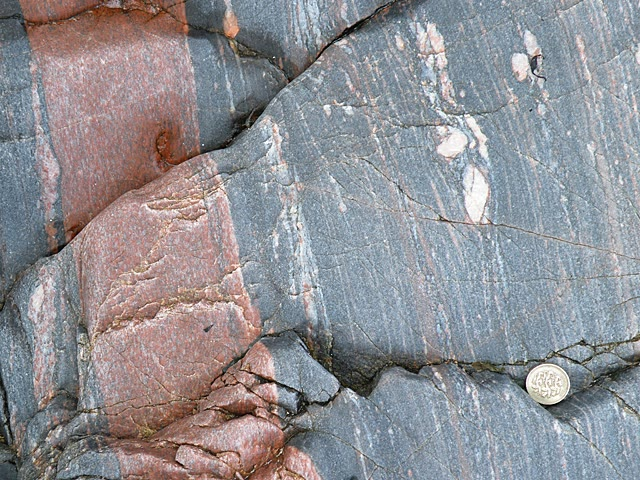
\includegraphics[width=0.5\linewidth]{images/book4/b2-12-leucogranite-vein.jpg}
\par\smallskip{\small Un filon de \omterm{def:b2:crustal-melting:leucogranite}{leucogranite} rose qui recoupe un gneiss gris rubané~; la pièce donne
l'échelle. Photographie Anne Burgess (Geograph), CC BY-SA 2.0.}
\end{omfigure}

\section{Granites et croissance des continents}\label{sec:b2:crustal-melting:time}

Deux types de lieux produisent l'essentiel du granite. Au-dessus des zones de subduction, la croûte d'arc se forme par
différenciation de liquides mafiques issus du manteau, et la chaleur disponible est seulement celle que ces
liquides apportent. Après une collision, la croûte épaissie est un système très chaud~: elle fond à grande
échelle, à basse température là où l'eau ou la muscovite le permet, et à plus haute température par la
décomposition de la biotite, et ces granites issus de la croûte recyclent une croûte qui existait déjà.
Les liquides mantelliques atteignent aussi la croûte là, en quantités assez grandes, selon Moyen et
ses collaborateurs, pour faire des ceintures tardi-orogéniques un contributeur important à la croissance
de la croûte. Qu'un granite ajoute à la croûte continentale ou se contente de la remanier relève donc
de sa source, que ses isotopes permettent de déterminer (\cref{ch:b2:isotope-geochemistry})~; les granites de
la Terre primitive, très différents de ceux-ci, font l'objet du
\cref{ch:b2:precambrian-earth}.
% ledger: moyen17:settings

\section{Exercices}\label{sec:b2:crustal-melting:exercises}

Masses molaires (\unit{\gram\per\mole})~: \ce{Al2O3} 101.96, \ce{CaO} 56.08, \ce{Na2O} 61.98,
\ce{K2O} 94.20, \ce{H2O} 18.02~; masses atomiques~: H 1.008, O 16.00, Na 22.99, Mg 24.31,
Al 26.98, Si 28.09, K 39.10, Ca 40.08. Prendre $g = \qty{9.81}{\metre\per\second\squared}$.

\begin{exercise}[$\star$]\label{exo:b2:crustal-melting:1}
Le matériau de référence andésitique AGV-2 contient, en \unit{\gram} pour \qty{100}{\gram},
\ce{Al2O3} 17.03, \ce{CaO} 5.15, \ce{Na2O} 4.204 et \ce{K2O} 2.898.
(a) Calculer son A/CNK et son A/NK. (b) Classer la roche, et nommer un minéral qui doit porter son
calcium en excès.
\end{exercise}
% ledger: usgs:agv2-major

\begin{exercise}[$\star$]\label{exo:b2:crustal-melting:2}
Trois granites contiennent, outre le quartz et les feldspaths~: (a) muscovite, biotite et grenat~;
(b) hornblende, biotite et titanite~; (c) égirine, un pyroxène sodique--ferrique
\ce{NaFeSi2O6}, et une amphibole sodique. Classer chacun selon sa saturation en aluminium, et dire
lequel pourrait être un \omterm{def:b2:crustal-melting:types}{granite de type S}.
\end{exercise}

\begin{exercise}[$\star$]\label{exo:b2:crustal-melting:3}
Une croûte de masse volumique \qty{2800}{\kilogram\per\cubic\metre} a un géotherme linéaire
$T = \qty{10}{\celsius} + (\qty{20}{\celsius\per\kilo\metre})\,z$. Entre 2 et
\qty{10}{kbar}, approcher le solidus humide du granite par la droite passant par
(\qty{680}{\celsius}, \qty{2}{kbar}) et (\qty{620}{\celsius}, \qty{10}{kbar}). À quelle
profondeur, quelle température et quelle pression le géotherme rencontre-t-il ce solidus~?
\end{exercise}
% ledger: sw81:wet-solidus

\begin{exercise}[$\star$]\label{exo:b2:crustal-melting:4}
Un gneiss gris à biotite porte des couches blanches de quartz et de feldspath, d'un centimètre d'épaisseur,
parallèles à sa foliation, chacune bordée d'un fin liséré noir de biotite~; entre les couches, le gneiss
paraît ordinaire. (a) Nommer les couches blanches, les liserés noirs et le gneiss ordinaire. (b) La roche
est-elle une \omterm{def:b2:crustal-melting:migmatite}{métatexite} ou une \omterm{def:b2:crustal-melting:migmatite}{diatexite}, et quelle est sa structure~? (c) À quelques centaines de
mètres de là, la stratification a disparu~: une roche striée, d'aspect granitique, porte des fantômes
pâles de gneiss. Qu'est-ce qui a changé~?
\end{exercise}
% ledger: scmr:migmatite, bgs99:migmatite

\begin{exercise}[$\star\star$]\label{exo:b2:crustal-melting:5}
Prenons la biotite comme phlogopite, \ce{KMg3AlSi3O10(OH)2}. (a) Calculer sa masse molaire et la
fraction massique d'eau qu'elle libère (ses deux groupes hydroxyle donnent un \ce{H2O}).
(b) Un gneiss à \qty{25}{\percent} de biotite en masse fond par \omterm{def:b2:crustal-melting:reactions}{fusion par déshydratation} de la biotite
en un liquide qui contient \qty{4.0}{\percent} d'eau. En utilisant la
\cref{prop:b2:crustal-melting:water}, trouver le \omterm{def:b2:mantle-melting:fraction}{taux de fusion}, et le comparer aux
fractions observées dans les expériences de \omterm{def:b2:crustal-melting:reactions}{fusion par déshydratation} de la biotite.
\end{exercise}
% ledger: bk99:migmatites

\begin{exercise}[$\star\star$]\label{exo:b2:crustal-melting:6}
Cent grammes de granite contiennent \qty{30}{\gram} de feldspath potassique \ce{KAlSi3O8},
\qty{35}{\gram} d'albite \ce{NaAlSi3O8}, \qty{5}{\gram} d'anorthite \ce{CaAl2Si2O8},
\qty{25}{\gram} de quartz et \qty{5}{\gram} de muscovite \ce{KAl3Si3O10(OH)2}.
(a) Calculer les masses molaires des quatre minéraux alumineux. (b) Calculer les quantités de
\ce{Al2O3}, \ce{CaO}, \ce{Na2O} et \ce{K2O} dans la roche, et son A/CNK. (c) Quel
minéral rend la roche \omterm{def:b2:crustal-melting:asi}{hyperalumineuse}~?
\end{exercise}

\begin{exercise}[$\star\star$]\label{exo:b2:crustal-melting:7}
Un \omterm{def:b2:magma-emplacement:bodies}{sill} basaltique intrudé à \qty{1200}{\celsius} cristallise complètement et se refroidit jusqu'à
\qty{850}{\celsius}, en libérant une chaleur latente de \qty{900}{\mega\joule\per\cubic\metre}.
La croûte qui l'entoure, à \qty{650}{\celsius}, est chauffée jusqu'à \qty{850}{\celsius} et
\qty{20}{\percent} de son volume fond, avec la même chaleur latente par unité de volume de liquide. Les deux
roches ont une capacité calorifique de \qty{2.5}{\mega\joule\per\cubic\metre\per\kelvin}. En utilisant
la \cref{prop:b2:crustal-melting:heat}, combien de mètres cubes de croûte un mètre cube de basalte peut-il
traiter de cette façon~? Qu'est-ce que le résultat ignore~?
\end{exercise}
% ledger: delaney86b4:properties

\begin{exercise}[$\star\star$]\label{exo:b2:crustal-melting:8}
Le matériau de référence obsidienne SRM 278 est certifié à \ce{Al2O3}
$14.15 \pm 0.15$, \ce{CaO} 0.983, \ce{Na2O} 4.84 et \ce{K2O} 4.16 (\unit{\percent} en
masse). (a) Calculer son A/CNK et son A/NK, et la classer. (b) Recalculer A/CNK avec les deux
bornes de l'incertitude sur \ce{Al2O3}. La classification est-elle robuste~?
\end{exercise}
% ledger: nist278:majors

\begin{exercise}[$\star\star$]\label{exo:b2:crustal-melting:9}
À \qty{800}{\celsius}, un liquide haplogranitique saturé en eau contient \qty{7.45}{\percent}
d'eau à \qty{3}{kbar}, 8.94 à \qty{4}{kbar}, 9.97 à \qty{5}{kbar} et 13.82 à
\qty{8}{kbar}. (a) Ajuster une droite à ces quatre points par moindres carrés et comparer
sa pente avec les \qty{1.27}{\percent} par kilobar donnés par les expérimentateurs.
(b) Prédire la teneur de saturation à \qty{6}{kbar}. (c) Quelle est la masse minimale de liquide
qui peut porter \qty{10}{\gram} d'eau à \qty{6}{kbar}~? (d) Pourquoi la droite ne doit-elle pas
être utilisée à \qty{15}{kbar}~?
\end{exercise}
% ledger: holtz95:solubility

\begin{exercise}[$\star\star\star$]\label{exo:b2:crustal-melting:10}
Approcher le solidus de \omterm{def:b2:crustal-melting:reactions}{fusion par déshydratation} d'un schiste à muscovite par la droite passant par
(\qty{750}{\celsius}, \qty{6}{kbar}) et (\qty{800}{\celsius}, \qty{10}{kbar}),
les extrémités des encadrements expérimentaux. Un schiste à \qty{770}{\celsius} remonte depuis
\qty{10}{kbar} sans gagner ni perdre de chaleur. (a) À quelle pression atteint-il le
solidus~? (b) Au-delà, sa température suit le solidus vers le bas, la chaleur de fusion provenant
de son propre refroidissement. Avec une capacité calorifique de \qty{2.5}{\mega\joule\per\cubic\metre\per\kelvin}
et une chaleur latente de \qty{900}{\mega\joule\per\cubic\metre}, quelle fraction volumique de liquide
s'est formée lorsqu'il atteint \qty{6}{kbar}~? (c) Comparer avec les conditions proposées pour
les \omterm{def:b2:crustal-melting:leucogranite}{leucogranites} de l'Himalaya.
\end{exercise}
% ledger: pdh98:himalaya, delaney86b4:properties

\begin{exercise}[$\star\star\star$]\label{exo:b2:crustal-melting:11}
La chaleur diffuse sur une distance $\ell$ en un temps de l'ordre de $\ell^2/\kappa$. Avec
$\kappa = \qty{1e-6}{\square\metre\per\second}$, estimer le temps pour que la chaleur d'un
\omterm{def:b2:magma-emplacement:bodies}{sill} de \qty{2}{km} d'épaisseur, et celle d'une couche sous-plaquée de \qty{10}{km}, se répande sur leur
propre épaisseur. Comparer avec les dix Ma de l'\omterm{def:b2:crustal-melting:anatexis}{anatexie} himalayenne~: un seul événement de sous-placage peut-il
l'expliquer~?
\end{exercise}
% ledger: delaney86b4:properties, weinberg16:himalaya

\begin{exercise}[$\star\star\star$]\label{exo:b2:crustal-melting:12}
Une \omterm{def:b2:crustal-melting:migmatite}{migmatite} stromatique est analysée~: \omterm{def:b2:crustal-melting:migmatite}{leucosome} \ce{K2O} \qty{5.0}{\percent}, \ce{MgO}
\qty{0.20}{\percent}~; \omterm{def:b2:crustal-melting:migmatite}{mélanosome} \ce{K2O} \qty{2.0}{\percent}, \ce{MgO}
\qty{4.0}{\percent}~; mésosome, pris comme roche mère non fondue, \ce{K2O}
\qty{2.75}{\percent}, \ce{MgO} \qty{3.05}{\percent} (toutes en masse). (a) Si le
néosome s'est formé à partir de la roche mère sans gain ni perte, quelle fraction massique du néosome est
\omterm{def:b2:crustal-melting:migmatite}{leucosome}~? (b) Vérifier la réponse avec \ce{MgO}. (c) Sur l'affleurement, le \omterm{def:b2:crustal-melting:migmatite}{leucosome} ne représente que
\qty{10}{\percent} du néosome en masse. Combien de grammes de liquide ont quitté
\qty{100}{\gram} de roche mère~?
\end{exercise}

\begin{problem}[{Problème du week-end --- un pluton issu d'un mica fondu}]\label{pb:b2:crustal-melting:1}
Un schiste formé de \qty{20}{\percent} de muscovite, \qty{15}{\percent} de biotite,
\qty{30}{\percent} de quartz, \qty{30}{\percent} de plagioclase et \qty{5}{\percent} d'autres
minéraux (en masse~; une roche fictive) se trouve à la base d'une croûte doublée par empilement, la situation modélisée au
\cref{ch:b2:pt-paths}. Il peut fondre et alimenter un \omterm{def:b2:magma-emplacement:bodies}{pluton} de granite. Données~: les masses
atomiques et molaires en tête des exercices~; le solidus humide du granite passe par
(\qty{680}{\celsius}, \qty{2}{kbar}), (\qty{620}{\celsius}, \qty{10}{kbar}),
(\qty{605}{\celsius}, \qty{15.3}{kbar}) et (\qty{670}{\celsius}, \qty{27}{kbar})~; la teneur
en eau de saturation d'un liquide granitique à \qty{800}{\celsius} est de \qty{9.97}{\percent} à
\qty{5}{kbar} et \qty{13.82}{\percent} à \qty{8}{kbar}. La base modèle de la croûte épaissie suit~:

\smallskip
\begin{center}\small
\begin{tabular}{l|ccccccccccc}
$t$ (\unit{Ma}) & 0 & 10 & 20 & 30 & 40 & 50 & 60 & 70 & 80 & 90 & 100\\ \hline
$T$ (\unit{\celsius}) & 595 & 656 & 734 & 795 & 845 & 885 & 909 & 914 & 900 & 867 & 814\\
$P$ (\unit{kbar}) & 19.2 & 19.2 & 19.2 & 19.2 & 17.9 & 16.5 & 15.1 & 13.7 & 12.4 & 11.0 & 9.6
\end{tabular}
\end{center}
\smallskip

\noindent\textbf{Partie I --- L'eau du mica.}
\begin{enumerate}
\item Calculer la masse molaire de la muscovite \ce{KAl3Si3O10(OH)2}.
\item Ses deux groupes hydroxyle donnent un \ce{H2O}. Quelle fraction massique du minéral est
libérée sous forme d'eau~?
\item Quelle quantité d'eau la muscovite d'un kilogramme de schiste libère-t-elle~?
\item En interpolant linéairement, quelle est la teneur en eau de saturation du liquide à
\qty{7}{kbar}~? Quel est alors le \omterm{def:b2:mantle-melting:fraction}{taux de fusion} minimal que l'eau de la muscovite peut produire~?
\item Le liquide de la \omterm{def:b2:crustal-melting:reactions}{fusion par déshydratation} est loin d'être saturé~; supposer sa teneur en eau égale à
\qty{6.0}{\percent}. Quel \omterm{def:b2:mantle-melting:fraction}{taux de fusion} la muscovite produit-elle~?
\item Dans les expériences sur une \omterm{def:b2:metamorphic-facies:protoliths}{métapélite} à deux micas à \qty{10}{kbar}, la réaction de la muscovite
n'a donné que 1 à \qty{2}{\percent} de liquide. Citer deux raisons pour lesquelles une roche réelle peut produire moins
de liquide que votre réponse à la question~5.
\end{enumerate}

\noindent\textbf{Partie II --- Chauffer la source.}
\begin{enumerate}[resume]
\item Au \cref{ch:b2:pt-paths}, la roche restée à mi-croûte culmine à \qty{593}{\celsius}
et \qty{7.8}{kbar}. Quel est le solidus humide à \qty{7.8}{kbar}~? Cette roche peut-elle fondre, même
en présence d'eau libre~?
\item En interpolant entre 15.3 et \qty{27}{kbar}, trouver le solidus humide à la pression
de la base juste après l'empilement. La base est-elle au-dessus à $t = 0$~? À $t = \qty{10}{Ma}$~?
\item Qu'est-ce qui limite la fusion de la base à $t = \qty{10}{Ma}$, et pourquoi s'arrête-t-elle
bientôt~?
\item Quand la base dépasse \qty{800}{\celsius}, borne haute de l'encadrement de la
muscovite~?
\item L'encadrement de l'amphibole s'étend de 875 à \qty{925}{\celsius} pour 10 à \qty{12.5}{kbar}.
Quand la base entre-t-elle dans cette gamme de pression, et à quelle température~?
\item Quand la base atteint-elle \qty{10}{kbar}, borne haute de la gamme de pression des
expériences sur la muscovite, et quelle température a-t-elle alors~? Quels minéraux hydratés du schiste peuvent
encore exister~?
\end{enumerate}

\noindent\textbf{Partie III --- Quel liquide~?}
Le liquide, une fois cristallisé, donne un \omterm{def:b2:crustal-melting:leucogranite}{leucogranite} (analyse fictive) contenant, en
\unit{\percent} en masse, \ce{Al2O3} 15.0, \ce{CaO} 0.55, \ce{Na2O} 3.4 et \ce{K2O} 4.9.
\begin{enumerate}[resume]
\item Calculer les quantités des quatre oxydes dans \qty{100}{\gram} de roche.
\item Calculer son A/CNK.
\item Calculer son A/NK et classer le \omterm{def:b2:crustal-melting:leucogranite}{leucogranite}.
\item S'agit-il d'un \omterm{def:b2:crustal-melting:types}{granite de type I} ou de type S~? Citer deux minéraux qui doivent porter son excès
d'aluminium~?
\item Combien de moles de \ce{Al2O3} par \qty{100}{\gram} restent après les
feldspaths~? Si tout ce surplus entrait dans la muscovite, qui porte un \ce{Al2O3} de plus par
formule que le feldspath potassique, combien de grammes de muscovite
contiendraient \qty{100}{\gram} de granite~?
\item L'obsidienne SRM 278 a un A/CNK $= 0.993$. Le \omterm{def:b2:crustal-melting:leucogranite}{leucogranite} et l'obsidienne peuvent-ils
provenir du même type de source~?
\end{enumerate}

\noindent\textbf{Partie IV --- Quelle quantité de croûte~?}
Un \omterm{def:b2:magma-emplacement:bodies}{pluton} fictif de ce \omterm{def:b2:crustal-melting:leucogranite}{leucogranite} a un volume de \qty{1000}{\cubic\kilo\metre}.
Prendre \qty{2650}{\kilogram\per\cubic\metre} pour le granite et
\qty{2800}{\kilogram\per\cubic\metre} pour le schiste~; supposer que \qty{70}{\percent} du
liquide quitte sa source et que toute l'eau du liquide s'échappe lors de sa cristallisation.
\begin{enumerate}[resume]
\item Quelle est la masse du \omterm{def:b2:magma-emplacement:bodies}{pluton}~?
\item Quelle masse de liquide (avec ses \qty{6.0}{\percent} d'eau) a-t-il fallu~?
\item En utilisant le \omterm{def:b2:mantle-melting:fraction}{taux de fusion} de la question~5, quelle masse de schiste a dû fondre~?
\item Quel volume de schiste cela représente-t-il~?
\item Si la source était une couche de \qty{5}{km} d'épaisseur, sur quelle surface a-t-elle fondu~?
\item Avec le \omterm{def:b2:mantle-melting:fraction}{taux de fusion} minimal de la question~4 à la place, de combien la source serait-elle plus grande~?
Donner le volume de croûte source fondu pour faire le \omterm{def:b2:magma-emplacement:bodies}{pluton}, en
\unit{\cubic\kilo\metre}, d'après la question~22.
\end{enumerate}
\end{problem}
